\section* {1.1  LU -  разложение матриц}

\subsection{Постановка задачи}
Реализовать алгоритм LU -  разложения матриц (с выбором главного элемента) в виде программы. Используя разработанное программное обеспечение, решить систему линейных алгебраических уравнений (СЛАУ). Для матрицы СЛАУ вычислить определитель и обратную матрицу. 

{\bfseries Вариант:} 12

\begin{cases}
& -x_1-8x_2+5x_4 = -60 \\
& 6x_1-6x_2+2x_3+4x_4 = -10 \\
& 9x_1-5x_2-6x_3+4x_4 = 65 \\
& -5x_1-9x_3+x_4 = 18 \\
\end{cases}
%\pagebreak

\subsection{Результаты работы}
\begin{figure}[h!]
\centering
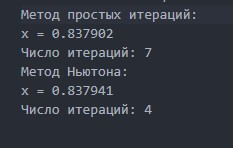
\includegraphics[width=15cm, height=10cm]{img1}
\caption{Вывод программы в консоли}
\end{figure}
\pagebreak

\subsection{Исходный код}
Файл с первым заданием лабораторной работы:
\lstinputlisting{include/task1.cpp}
\pagebreak
\section* {1.2  Метод прогонки}

\subsection{Постановка задачи}
Реализовать метод прогонки в виде программы, задавая в качестве входных данных ненулевые элементы матрицы системы и вектор правых частей. Используя разработанное программное обеспечение, решить СЛАУ с трехдиагональной матрицей.  

{\bfseries Вариант:} 12

\begin{cases}
& -11x_1+9x_2 = -114 \\
& x_1-8x_2+x_3 = 81 \\
& -2x_2-11x_3+5x_4= -8 \\
& 3x_3-14x_4+7x_5 = -38 \\
& 8x_4+10x_5 = 144\\
\end{cases}
% \pagebreak

\subsection{Результаты работы}
\begin{figure}[h!]
\centering
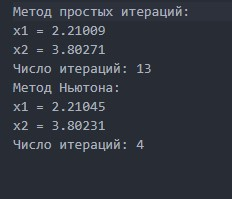
\includegraphics[width=.7\textwidth]{img2}
\caption{Вывод программы в консоли}
\end{figure}
\pagebreak

\subsection{Исходный код}
Файл со вторым заданием лабораторной работы:
\lstinputlisting{include/task2.cpp}
\pagebreak
\section* {1.3  Метод простых итераций. Метод Зейделя}

\subsection{Постановка задачи}
Реализовать метод простых итераций и метод Зейделя в виде программ, задавая в качестве входных данных матрицу системы, вектор правых частей и точность вычислений. Используя разработанное программное обеспечение, решить СЛАУ. Проанализировать количество итераций, необходимое для достижения заданной точности. 

{\bfseries Вариант:} 12

\begin{cases}

& 14x_1-4x_2-2x_3+3x_4 = 38 \\
& -3x_1+23x_2-6x_3-9x_4 = -195 \\
& -7x_1-8x_2+21x_3-5x_4 = -27 \\
& -2x_1-2x_2+8x_3+18x_4 = 142 \\
\end{cases}
% \pagebreak

\subsection{Результаты работы}
\begin{figure}[h!]
\centering
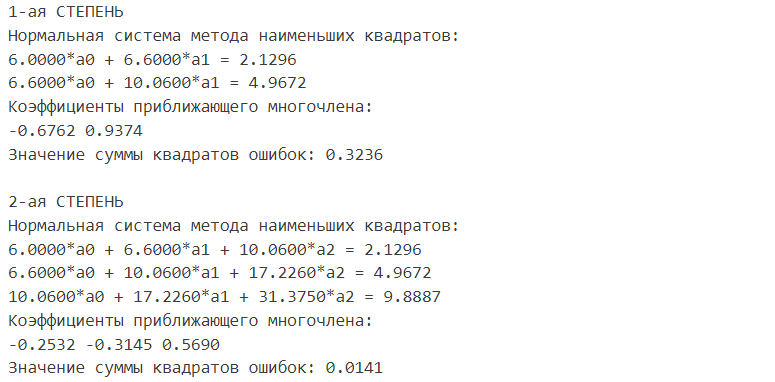
\includegraphics[width=15cm, height=10cm]{img3}
\caption{Вывод программы в консоли}
\end{figure}

% \vfill

\pagebreak

\subsection{Исходный код}
Файл с третьим заданием лабораторной работы:
\lstinputlisting{include/task3.cpp}
\pagebreak
\section* {1.4  Метод вращений}

\subsection{Постановка задачи}
Реализовать метод вращений в виде программы, задавая в качестве входных данных матрицу и точность вычислений. Используя разработанное программное обеспечение, найти собственные значения и собственные векторы симметрических матриц. Проанализировать зависимость погрешности вычислений от числа итераций. 

{\bfseries Вариант:} 12

  \begin{pmatrix}
    7 & 3 & -1 \\
    3 & -7 & -8 \\
    -1 & -8 & -2
  \end{pmatrix}
% \pagebreak

\subsection{Результаты работы}
\begin{figure}[h!]
\centering
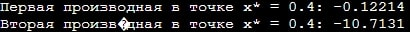
\includegraphics[width=.9\textwidth]{img4}
\caption{Вывод программы в консоли}
\end{figure}

\pagebreak

\subsection{Исходный код}
Файл с четвертым заданием лабораторной работы:
\lstinputlisting{include/task4.cpp}
\pagebreak
\section* {1.5  QR – разложение матриц}

\subsection{Постановка задачи}
Реализовать алгоритм QR – разложения матриц в виде программы. На его основе разработать программу, реализующую QR – алгоритм решения полной проблемы собственных значений произвольных матриц, задавая в качестве входных данных матрицу и точность вычислений. С использованием разработанного программного обеспечения найти собственные значения матрицы.


{\bfseries Вариант:} 12

  \begin{pmatrix}
    5 & -1 & -2 \\
    -4 & 3 & -3 \\
    -2 & -1 & 1
  \end{pmatrix}
% \pagebreak

\subsection{Результаты работы}
\begin{figure}[h!]
\centering
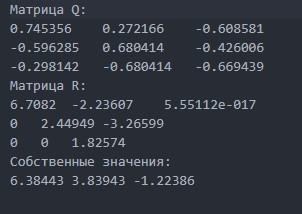
\includegraphics[width=.9\textwidth]{img5}
\caption{Вывод программы в консоли}
\end{figure}

\pagebreak

\subsection{Исходный код}
Файл с пятым заданием лабораторной работы:
\lstinputlisting{include/task5.cpp}